
\subsection{Convolutional Autoencoder with LSTM}
\label{section:Discussion:Discussion:CNN-AE-LSTM}

% TODO
% - Why was the model selected?
% - Regarding the different datasets -> Does it make sense to use this model? (Is there high noise)
% - What are the results for the different data-sets (dataset 1, 2 and 3)
% - What model should performe better than others, and why?
% --> Do we have background theory to back this up?
% --> Does it make sense?
% --> 


% What was the aim of the experiments?
% --> Apply the CNN-AE and LSTM model to a new dataset with real world applicaitons
% --> Verrify the ability of ther hybrid model against the baseline LSTM
% --> Thus verrifying the claims done by "Zhao2019"
\todo[inline]{Trenger vi å oppsumere i så mye detalj her? Jeg har ikke gjort det tidligere.}
Inspired by the work done by \cite{Zhao2019}, the hybrid model CNN-AE and LSTM was selected.
The paper we base this work on explores the hybrid model's ability to make time series predictions
on data with a high noise.
This is due to the first part of the model, the convolutional autoencoder.
The autoencoder is added in an attempt to reduce the noise contained in the data before the data is passed through to the LSTM model.
With the results from the paper by \cite{Zhao2019} claim the hybrid model vastly improves the predictions made, reducing the loss value with
several percentage points over a standard LSTM model, the hope was that this could be verified on the real-world practical application of
predicting trend at ``Prisguiden.no''.
The experiments done with the autoencoder is therefore compared to the baseline LSTM model to explore and verify the claims done by
\cite{Zhao2019}.

% Link this to RQ-5 (CNN-AE and LSTM against the baseline LSTM)
% The paper is based on "Local univariate" models. We therefor first mention this
% All withing the margin of error
% We are not able to recreate the values by Zhao2019

% ....
% Dataset   -   LSTM   -  CNN
% Dataset 1 -  0.239   -  0.208 ->  13.9%
% Dataset 2 -  0.633   -  0.716 ->  -12.3%
% Dataset 3 -  0.488   -  0.483 ->  1%
After doing experiments with the LSTM and the CNN-AE and LSTM model on the three datasets used in this paper,
the results from the predictions is pressented in \cref{section:Results}.
Using the hybrid model, it is clear that we are not able to recreate the values presented in \cite{Zhao2019}
with all the different datasets.
The experiments conducted on the different datasets vary vastly between the hybrid and LSTM models.
While the CNN-AE-LSTM proves to have a bit more difficulties on dataset 2, and minor improvements on dataset 3,
it does, on average result in vast improvements on predictions done on dataset 1.
Using the hybrid model on dataset 1, the loss metrics for predictions are on average reduced with 13.9\% using the sMAPE metric.
In contrast, predictions made on dataset 2 result in forecasts that, on average, are 12.3\% worse than the standard LSTM.
Lastly, predictions made on dataset 3 only improves with 1\%.

% Why is this?
% --> Why is it only better on dataset 1, and much worse on dataset 2
% --> Can the dataset have something to do with this?
% --> What is with the dataset from the Zhao2019 paper? Is this a lot easier? Is there more unneeded noise data?
The reasons behind the varying predictive ability of the convolutional autoencoder and LSTM lies partially
in the properties of the different datasets.
Although datasets 1 and 2 were selcted due to the autocorrelation between the time series within the datasets,
they also have other abilities that differentiate the two.
\todo[inline]{What differentiate dataset 1 and 2? Summary and reference data section}
\todo[inline]{Why is the model so much beter on dataset 1, and so much worse on dataset 2?}
\todo[inline]{Why do we get the results we do? Is there any reason behind it?}





% We have now seen how it works on univariate local models
% We use new models, exploring multivariate and global
% It is not always better in these cases
% How do we explain this?
% Can we compare directly with the work done in Zhao2019? What error metrics were used in these models?
While the paper \cite{Zhao2019} only focuses on applying local univariate models,
we wished to explore the expansion of the use of the hybird model with other configurations.
These inclde the use of multivariate models and global models for each dataset.
Exploring the use of such variations to the Convolutional autoencoder and LSTM,
we hoped to uncover cases where the model performance is increased over the standard local uniariate model.



\subsubsection{Global univariate models}
% First -> Use of global models
% -> How does the global models performe in comparison to the LSTM version
% -> How does the global models performe in comparison to the local univariate standard model?

% Unødvendig gjentagelse?
%The first model variation that was tested were the use of a gloal univariate model.
%Both the LSTM model and the hybird convolutional autoencoder and LSTM model were tested on the same datasets,
%and with the same global univariate configuration.
%This is done in order to be able to compare the global univariate hybrid model both to the local univariate model,
%but also with the correlating global univariate LSTM model.

% ....
% Dataset   -   LSTM   -  CNN
% Dataset 1 -  0.203   -  0.210   ->  -3.4 %
% Dataset 2 -  0.662   -  0.675   ->  -1.9%
% Dataset 3 -  0.464   -  0.417   ->  10.7 %

\todo[inline]{Update after T tests results arrive}
The results on dataset 1 for the local univariate and the local multivariate models
confirms our hypothesis presented in RQ5 [\ref{G&R:RQ-CNN-AE-LSTM}], that the
CNN-AE-LSTM does achieve higher accuracy over a plain LSTM by a few percentage points.

The only exception is for the global models, where the CNN-AE-LSTM in general performs worse.
It seems the benefits of a global model for RNNs are not transferable to other types
of NNs. LSTMs ability to learn across multiple time series can be attributed to the fundamentals
of how the LSTM works. \cite{Zhao2019} discusses previous work that concludes that
the LSTMs memory cell is mainly responsible for the performance of the LSTM.
When training the LSTM on multiple time series, this memory cell is local to each
time series and resets before each new time series is fed through the network.
The LSTM weights on the other hand are global across all the series.
These local and global characteristics are unique to RNNs, and can explain
why the Convolutional Autoencoder does not see the same benefits when trained on multiple
time series.

The results of Experiment 4 [\Cref{section:results:additional-experimental-plan:Experiment-4}],
and Experiment 1 shows a small increase in performance for the hybrid model on high variance datasets.
Even though these results are not statistically significant, the sample sizes were relatively small
(20 samples, and 7 samples), which might be too small to conclude when the
performance increase is low.

However, from the results of Experiment 4, we can empirically conclude that the CNN-AE-LSTM will
hurt the performance if the datasets contain small amounts of noise. This downside is much
worse than the potential performance gains on noisy datasets.
This can explain the poor results on dataset 2. Since dataset 2 contains a wide variety
of time series.




%Unlike the local univariate models described above, the hybrid model performe quite similar, although somewhat worse than the LSTM model
%on both dataset 1 and 2.
%However, dataset 3 offers an improvement of a little over 10\% of the sMAPE error metric by the hybrid model compared to the LSTM.
%
%The results from the global univarite model are somewhat unexpected.
%Dataset 1 and 2 were selected due to their contrast in corrolation between the time series in the dataset.
%Dataset 1 has time-series wich correlate the most with each other, while dataset 2 has time-series with the least ammount of correlating between them.
%Using an convolutional autoencoder and LSTM, it was expected that the additional data made available through the use of a global configuration
%whould be utilized in order to improve the abilities of the autoencoder.
%The autoencoder would have more data to work with in order to improve its encoding and reconstructing of data,
%and considering the data corrolated to some extend, dataset 1 should be easier to work with as much of the data corrolate.
%
%However, as the experiments have shown, both dataset 1 and 2 performes poorly, by beeing a little wors than a LSTM model with the same
%global univariate configuration.
%\todo[inline]{Why? Does it make sense that we get these results here?}
%\todo[inline]{How does the model compare with the basic local univariate hybird model?}





\subsubsection{Local multivariate models}

Afther the use of global models, a configuration of multivariate models were attempted.
Unlike the glboal models,
the number of data points are increased not through the addition of other time-series,
but by decomposing the information within each time-series to include seasonal values such as season or day of the week.

Using the convolutional autoencoder and LSTM model on this problem should result in both imporvements and degregation to performance.
Initially, the performance of the model should suffer due to the fact that the model is required to encode and reconstruct the
input data.
The model might encounter problems with recreating the data using the same model as for univariate models,
while attempting to recreate additional datapoints.
However, the same reasoning might also help improve the hybrid model's performance in some cases.
While more data need to be encoded and reconstructed, the autoencoder will retain more information
regarding the development of trends and spikes through different seasons.
% Den er ikke like grov i kantene
While a pattern migh repeat over several seasons, there migh be additional hidden information in the seasonal information.
If a pattern is known to never spike during summer but often spikes through the winter,
the autoencoder should be able to differentiate between the different seasons.
It would be more likely to accept the spikes during the winter as relevant information, while a random spike during the summer might be reduced.
This would mean that it would be more well adjusted to reduce noise in a pattern also dependent on the seasonal factors,
thus beeing more finly tuned for individual patterns.

% Second -> Use of local multivariate
% ....
% Dataset   -   LSTM   -  CNN
% Dataset 1 -  0.183   -  0.181  ->  1.1%
% Dataset 2 -  0.603   -  0.743  ->  -20.8%
% Dataset 3 -  0.325   -  0.354  ->  -8.5%
However, while this reasoning is based on the autoencoders ability to encode and differentiate between values based on season,
it model would be severly limited in cases where there is not enough data for the autoencoder to learn of such connections.
As discussed in \cref{section:Data:DataExploration}, the data attained from ``Prisguiden.no'' only include datapoints
for a little over 3 years.
Considering the limited information per datapoints, this amount of data could heavily limit the convolutional autoencoder and lstm model.
This is also reflected in the results aquired through testing.
While dataset 1 have a small improvement by the hybrid model with around 1\%,
the basic LSTM model heavily outperform the convolutional autoencoder and LSTM model by over 20\% for dataset 2, and over 8\% for dataset 3.

Although the local multivatiate model is the overall best performing of the convolutional autoencoder and LSTM models,
it is outperformed by the LSTM, indicating that the reason for the improvements by the model
is entirely contributed by the improvements to the LSTM model.
The results for these experiments are well withing the expected performance of the local multivariate model.
\todo[inline]{Jeg skjønner ikke helt argumentet her. CNN-AE-LSTM gjør det gjevnt over best på dataset 1, med untak av global univariate.
  At den gjør det dårligere på datset 2 kan forklares med at nedsiden til autoencoder er større en oppsiden, så noen få kan trekke ned snittet.
}





\subsubsection{Global Multivariate models}

Expanding on the use of global models and multivariate models,
a global multivariate hybrid model is defined and tested.

Even though the model is a global method; it does not escape the problems retained with a multivariate model.
Although the number of datasets has increased, this does not nessesarily improve the performance of the models.
The reason behind this is the lack of correlation between the time-series in the datasets.
Although dataset 1 contains datasets with higher correlation than dataset 2 and 3, it appears this is not enough to make any significant difference.
While it does performe 2\% better than the global mulitivariate LSTM, this is not enough to say that the autoencoder adds
in any meaningfull way.
When it comes to dataset 2 and 3 where the correlation between datasets is excedingly low, the autoencoder ends up with decreasing the performance of the predictions.
There might be several different factors that play a part in this.

Dataset 1 contains data with high correlation, and thus the autoencoder is more likely to use the additonal data to performe well with encoding and reconstruction.
However, it appears that the autoencoder is not able to improve predictions.
\todo[inline]{Why these reuslts? Are they expected?}


The results are different on datasets 2 and 3 however.
While dataset 1 showed little difference, dataset 2 and 3 performe much worse than the LSTM for a global multivariate model.
This could be explained by the low correlation between the data, which again could result in the autoencoder having to encode a lot more data,
without the performance advantage of analysing data that is shared accorss the time-series.
The autoencoder would therefor have more dificulties in encoding and reconstructing the data,
thus making error prone reconstructions and therefor hurting the performance of the model.
For dataset 2 and 3, these results are as expected for the global multivariate model.



% Has problems with multivariate values, just like the local multivariate
% Sum it up to be the same.
% Has the same advantages as the global univariate, but what were thos?


% Third -> Use of global multivariate
% ....
% Dataset   -   LSTM   -  CNN
% Dataset 1 -  0.202   -  0.198  ->  2%
% Dataset 2 -  0.642   -  0.703  ->  -9.1%
% Dataset 3 -  0.447   -  0.566  ->  -23.5%



\todo[inline]{Why? Does it make sense that we get these results here?}

\todo[inline]{How does the model compare with the basic local univariate hybird model?}







% Additional  ->  High variance vs low-variance datasets



% Old
\iffalse
  The CNN-AE-LSTM model is only the best performing model for one dataset, dataset 1.
  Here the CNN-AE-LSTM local multivariate model structure beat the plain local multivariate LSTM with $1.09\%$.
  The CNN-AE-LSTM performs competitively on all the experiments on dataset 1 except for the global univariate model structure.
  Our experiments show that adding a Convolutional Autoencoder to an LSTM can be beneficial in some scenarios.


  \begin{figure}[h!]
    \centering
    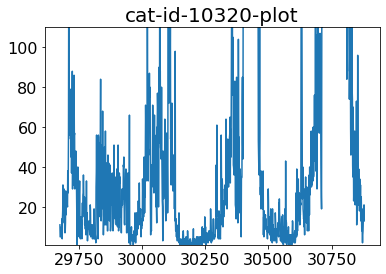
\includegraphics[width=\textwidth]{./figs/code_generated/data_exploration/cat-id-10320-plot.png}
    \hfill
    \caption{TODO}
    \label{fig:cat-id-10320-cnn-ae-beat-lstm}
  \end{figure}

  \import{./tables/results/dataset_high_variance}{Average-metric-dataset-high-variance.tex}

  \begin{figure}[h!]
    \centering
    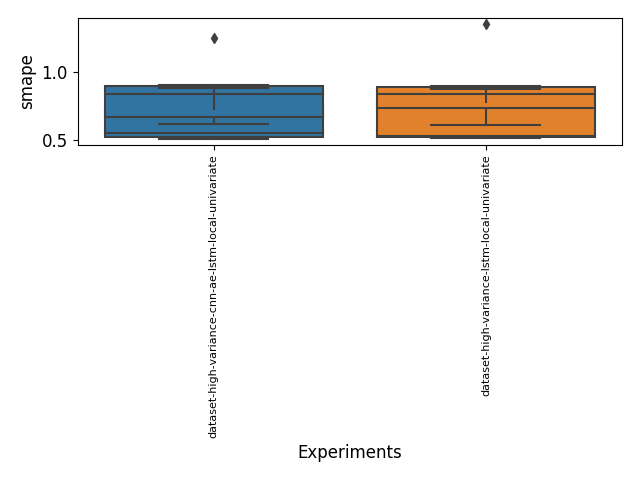
\includegraphics[width=\textwidth]{./figs/results/boxplot/smape-dataset_high_variance.png}
    \hfill
    \caption{TODO}
    \label{fig:results-smape-dataset-high-variance}
  \end{figure}
\fi
